We perform our analysis on the AOL query log~\cite{pass2006picture}, since it is easy to obtain\footnote{the query log can be retrieved from \url{http://www.gregsadetsky.com/aol-data/}}
AOL query log consists of approximately 20 millions of queries submitted by $650,000$ users from March to May in 2006. Queries are normalized (text lowercased, not ascii characters removed) and 
there are in total $10,154,742$ distinct queries. 

\begin{figure}
	\centering
	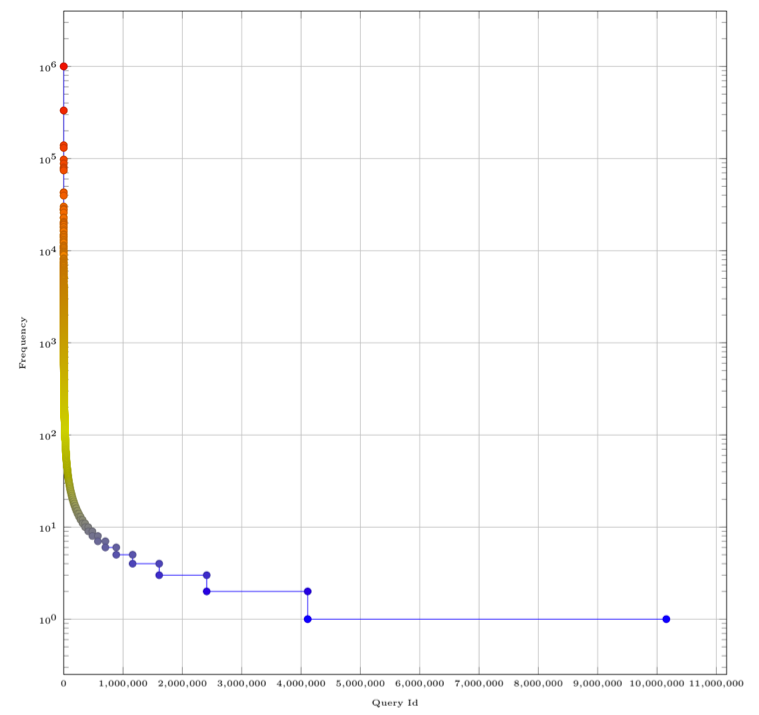
\includegraphics[scale=0.28]{images/aol}
	\caption{Query frequency distribution in AOL query log}
\end{figure}